\section*{Plan de Proyecto}

Considerando las posturas de los stakeholders con los que se tuvo contacto, se decidi\'o dar prioridad a la usabilidad, rendimiento, e integrabilidad y extensibilidad. Para esta segunda parte se cuenta con una dedicaci\'on \textit{full-time} de los tres integrantes del equipo.

\subsubsection{Iteraci\'on 1 - Elaboraci\'on (2 semanas / 240 horas)}	
	
	\begin{itemize}
		  \item Definici\'on de arquitectura
		  \item CU-01: Autentic\'andose al sistema
		  \item CU-02: Cargando oferta a trav\'es de la Web-API
		  \item CU-03: Consultando oferta a trav\'es de API-Internet
		  \item CU-04: Consultando oferta a trav\'es de p\'agina web TPA
		  \item CU-05: Enviando sugerencia sobre el sistema
	\end{itemize}

	Los casos de uso incluidos en esta primera iteraci\'on conforman un subconjunto m\'inimo que nos permite tener un recorrido completo de la aplicación. Esto \'ultimo implica tambi\'en que varios de \'estos tiene un alto impacto en la arquitectura, teniendo que tomar decisiones al respecto de la autenticaci\'on, implementaci\'on del servicio Web-API, integraci\'on del sitio Web-TPA con el servicio API, modelo de persistencia de entidades y resoluci\'on de b\'usquedas.
	
	Desde el punto de la usabilidad, incluimos el env\'io de sugerencia para tener un feedback temprano del usuario. Desde el punto de vista del rendimiento, apuntamos a utilizar una interfaz simple, que minimice el intercambio de datos por consulta. Por \'ultimo, desde el punto de vista de la integrabilidad y extensibilidad, decidimos implementar todos las funcionalidades en el servicio Web-API, reutilizándolo desde el sitio Web-TPA.
	
	\begin{figure}[hbtp]
	\centering
	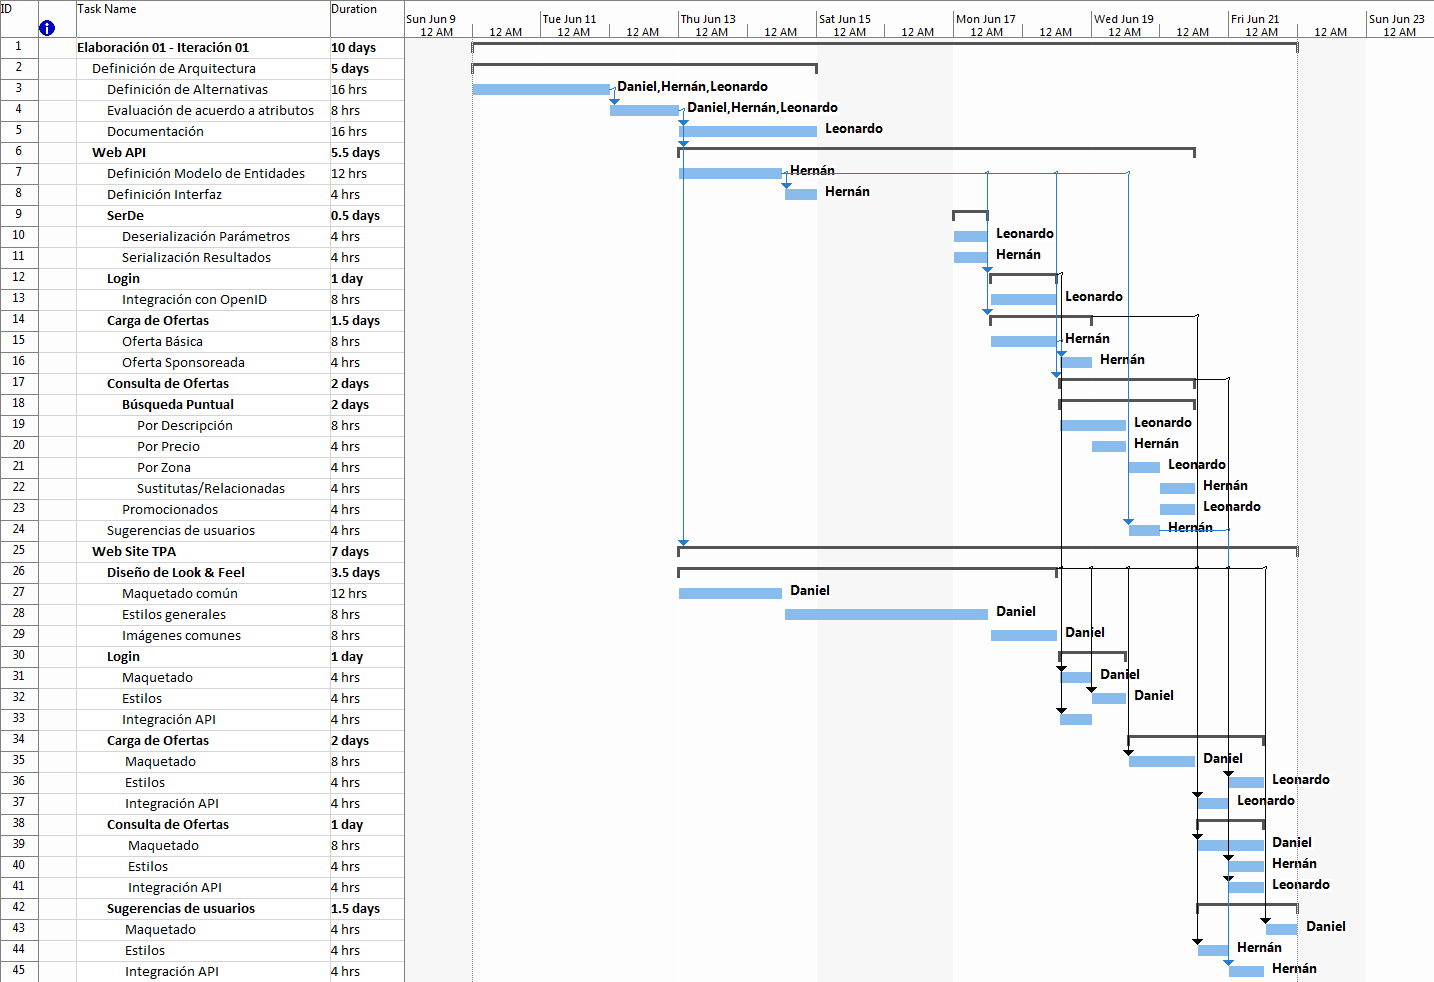
\includegraphics[scale=0.8]{./TP2Planificacion.gif}
	\caption{Diagrama de Gantt de tareas de la primera iteraci\'on, con divisi\'on de tareas y asignaci\'on de recursos}
	\label{fig:gantt}
	\end{figure}

\subsubsection{Iteraci\'on 2 - Elaboraci\'on (2 semanas / 240 horas)}
	
	\begin{itemize}
	  \item CU-06: Configurando oferta sugerida (24hs)
	  \item CU-07: Buscando información de oferta sugerida (32hs)
	  \item CU-08: Generando reporte de ofertas dudosas con Spam-Buster (64hs)
	  \item CU-09: Invalidando oferta (56hs)
	  \item CU-10: Cargando/Consultando oferta por P\'agina Web/Red Social [Twitter] (64hs)
	\end{itemize}

\subsubsection{Iteraci\'on 3 - Elaboraci\'on (2 semanas / 240 horas)}
	
	\begin{itemize}
		\item CU-10: Cargando/Consultando oferta por P\'agina Web/Red Social [cont.] (64hs)
		\item CU-11: Generando reporte de ofertas dudosas con M\'odulo Propio (64hs)
		\item CU-12: Registrar informacion de uso del sistema (24)
		\item CU-13: Asignando confiabilidad a oferta (48)
		\item CU-14: Asignando confiabilidad a usuario (40)
	\end{itemize}

\subsubsection{Iteraci\'on 4 - Construcci\'on (4 semanas / 480 horas)}
	
	Las siguientes tareas se desarrollan para finalizar con el deplyment del sistema
	
	\begin{itemize}
		  \item CU-10: Cargando/Consultando oferta por P\'agina Web/Red Social [cont.] (80hs)
		  \item CU-15: Comparando SpamBuster con Modulo de Ofertas dudosas (160hs)
		  \item CU-16: Configurando sistema de confianza personal (136hs)
		  \item CU-17: Mostrando mapa oferta (104hs)
	\end{itemize}

\subsubsection{Iteraci\'on 5 - Transici\'on (1 semana / 120 horas)}
	
	\begin{itemize}
		  \item CU-10: Cargando/Consultando oferta por P\'agina Web/Red Social [cont.] (40hs)
		  \item CU-18: Analizando web en busca de ofertas (48hs)
		  \item CU-18: Cargando/Consultando oferta por SMS (36hs)
	\end{itemize}
